\documentclass[a4paper]{article}

\usepackage[utf8]{inputenc}
\usepackage[english]{babel}

\usepackage{amsmath,amsthm,amssymb}
\usepackage{geometry} % for correct margins
\usepackage{graphicx}
\usepackage{listings}
\usepackage{hyperref}

\newcommand{\prog}[1]{\texttt{#1}}
\newcommand{\pfun}[1]{\textsf{#1}}

\lstset{basicstyle=\ttfamily,
frame=single,
language=C,
}

\title{Concurrency Theory, Assignment Lecture 5}
\author{Krasimir Georgiev}

\begin{document}
\maketitle

The following PGLEcw program \prog{Add} computes $x1 + x2$.
It increments $c1$ and decrements $c2$ until $c2$ becomes zero.
\lstinputlisting{Add}

The following PGLEcw program \prog{InitAdd} initializes the counters to
$c1 = 2, c2 = 3$.
\lstinputlisting{InitAdd}

The following PGLEcw program \prog{MultAdd} computes $x1 + x2 * x3$.
It adds $c2$ to $c1$ $c3$ times. Since the addition destructs the input value
of $c2$, it is stored in $t2$ and restored afterwards.
\lstinputlisting{MultAdd}

The following PGLEcw program \prog{XXaXa1} computes $x1^2 + x1 + 1$.
It copies $c1$ to $c2$ and $c3$, executes \prog{MultAdd} and increments the
result.
\lstinputlisting{XXaXa1}

The following PGLEcw program \prog{InitXXaXa1} initializes $c1 = 3$.
\lstinputlisting{InitXXaXa1}

The following is a screenshot of the simulator running \prog{XXaXa1} after
\prog{InitXXaXa1}.

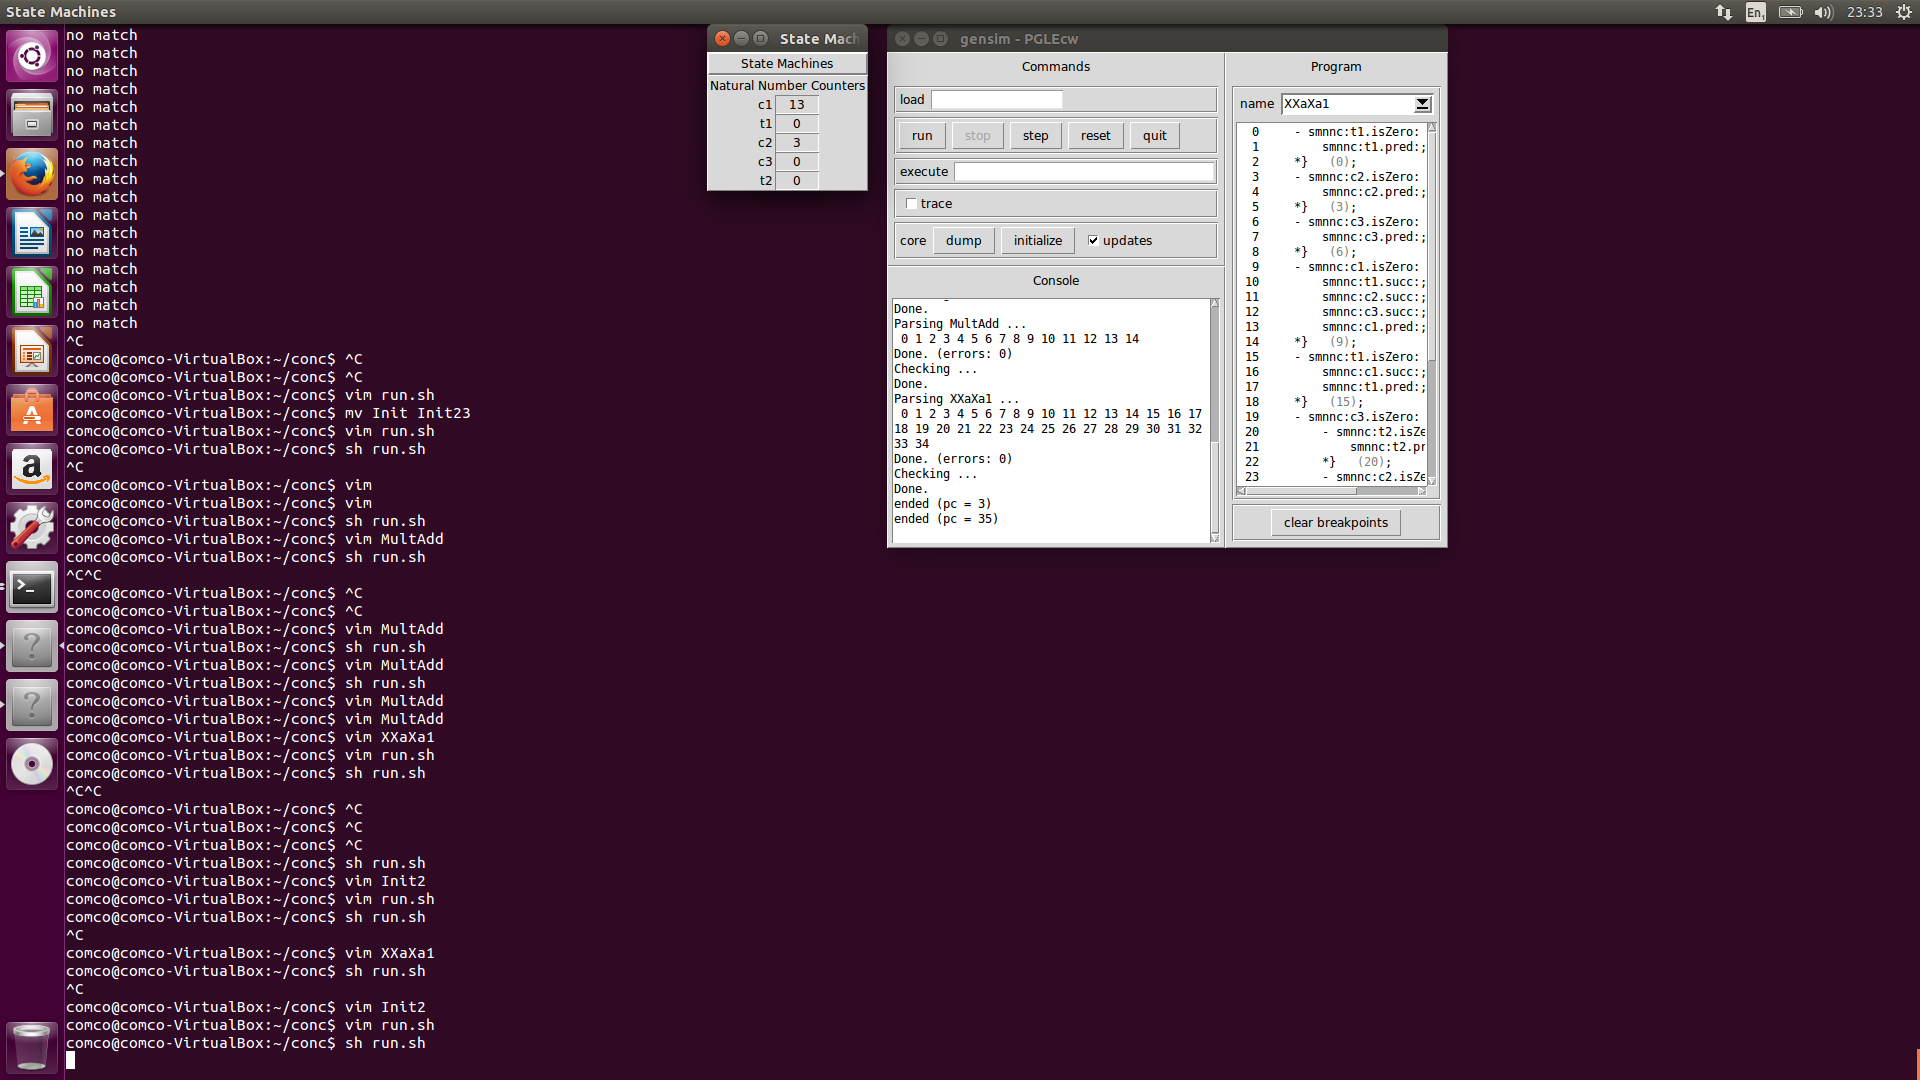
\includegraphics[scale=0.2]{assignment.png}

The programs are run using the following command:
\lstinputlisting[language=bash]{run.sh}

The source code of this assignment can be found on
\href{https://github.com/comco/concurrency-theory-assignments/tree/master/assignment-lecture-5}{GitHub}.
\end{document}
